\documentclass[conference]{IEEEtran}

\usepackage{graphicx}
\usepackage{subcaption}
\usepackage{amsmath} % assumes amsmath package installed
\usepackage{subcaption}
\usepackage{amssymb}
\usepackage{array}
\usepackage{tikz,circuitikz}
\usetikzlibrary{fit}
\usepackage{blindtext}
\usepackage{color}
\usepackage{siunitx}
\usepackage{float} % enables [H] float placement

\def\BibTeX{{\rm B\kern-.05em{\sc i\kern-.025em b}\kern-.08em
    T\kern-.1667em\lower.7ex\hbox{E}\kern-.125emX}}


\usepackage{mwe}
\usepackage{fancyhdr}
\fancypagestyle{firststyle}
{
	\fancyhf[C]{\fontsize{8}{10} \selectfont \textit{} }
	\fancyfoot[C]{}
}


\hyphenation{op-tical net-works semi-conduc-tor}


\begin{document}
%
% paper title
% Titles are only capitalized in the first letter.
% Linebreaks \\ can be used within to get better formatting as desired.
% Do not put math or special symbols in the title.
\title{Análisis de un rectificador de media onda con carga RL}

\author{
\IEEEauthorblockN{Yosniel Agüero}
\IEEEauthorblockA{\textit{Universidad de Guadalajara}\\
MCIE\\
Guadalajara, México\\
\scriptsize{\textit{yosniel.aguero9368@alumnos.udg.mx}}}
\and
\IEEEauthorblockN{Glader Hernandez}
\IEEEauthorblockA{\textit{Universidad de Guadalajara}\\
MCIE\\
Guadalajara, México\\
\scriptsize{\textit{glader.hernandez9367@alumnos.udg.mx}}}
\and
\IEEEauthorblockN{Gary Sosa}
\IEEEauthorblockA{\textit{Universidad de Guadalajara}\\
MCIE\\
Guadalajara, México\\
\scriptsize{\textit{gary.sosa9369@alumnos.udg.mx}}}
\and
\IEEEauthorblockN{Ulrik Wong}
\IEEEauthorblockA{\textit{Universidad de Guadalajara}\\
MCIE\\
Guadalajara, México\\
\scriptsize{\textit{ulrik.wong7998@alumnos.udg.mx}}}
}


\maketitle

\thispagestyle{firststyle}
\renewcommand{\headrulewidth}{0in}
\pagestyle{empty}


\pagestyle{fancy}
\chead{\fontsize{8}{10} \selectfont \textit{} }
\pagenumbering{gobble}



% As a general rule, do not put math, special symbols or citations
% in the abstract
\begin{abstract}
This document is a model and instructions for \LaTeX.
This and the IEEEtran.cls file define the components of your document [title, text, heads, etc.]. *CRITICAL: Do Not Use Symbols, Special Characters, Footnotes, 
or Math in Document title or Abstract.
\end{abstract}


\IEEEpeerreviewmaketitle



\section{Introduction}
This document is a model and instructions for \LaTeX.
Please observe the report page limits.
 
\begin{figure}[ht]
	\centering
	\begin{circuitikz}[american, cute inductors, american currents, american voltages]
		\ctikzset{diodes/scale=0.5, sources/scale=0.75, resistors/scale=0.5, inductors/scale=0.75}
		\draw (0,0) to[sinusoidal voltage source, v^<=$v_i$] (0,2) to [full diode, l_=$D_1$, v^=$v_{D}$, i_=$i_D$](2,2);
		\draw (2,0) to[full diode, l^=$D_2$, v_<=$v_{oi}$](2,2) to[L, l_=$L$, i_=$i_L$, v^=$v_L$] (4,2);
		\draw (4,2)-- (5,2) to[R, l_=$R$, v^=$v_R$, i>_=$i_R$] (5,0);
		\draw (0,0) -- (5,0);
	\end{circuitikz}
\end{figure}
\section{Análisis del rectificador monofásico de media onda con carga \(R\!-\!L\) y diodo de corrida libre}
La fuente sinusoidal de la entrada es: 
\[
v_i(t)=V_m\sin(\omega t),
\]
una impedancia serie \(R\) y \(L\) (carga), y dos diodos ideales:
\begin{itemize}
  \item \(D_1\): rectificador que conecta la fuente a la carga.
  \item \(D_2\): diodo de \emph{corrida libre} en paralelo a la carga.
\end{itemize}

\subsection{Estados asumidos de los diodos}

Definición de los 4 estados considerados y denotamos ON como  conducción (diodo polarizado directamente) y OFF como bloqueo (polarizado inversamente).
\[
\begin{array}{ll}
\text{Estado A: } & (D_1=\mathrm{ON},\; D_2=\mathrm{OFF}) \\
\text{Estado B: } & (D_1=\mathrm{OFF},\; D_2=\mathrm{ON}) \\
\text{Estado C: } & (D_1=\mathrm{OFF},\; D_2=\mathrm{OFF}) \\
\text{Estado D: } & (D_1=\mathrm{ON},\; D_2=\mathrm{ON}) \\
\end{array}
\]


\begin{itemize}
  \item \textbf{Operación de cada estado asumido :}
    \begin{enumerate}
      \item Estado A: Ocurre cuando la tensión instantánea de la fuente tiende a \emph{polarizar positivamente} \(D_1\) y puede imponer una tensión mayor en el nodo de carga que la necesaria para forzar \(D_2\) en conducción inversa. \(D_1\) conduce si \(\;v_i(t) > v_R(t)\) (ánodo de \(D_1\) más positivo que su cátodo). En la práctica, con diodos ideales y caída nula, el encendido ocurre cuando \(v_i(t)\) supera la tensión instantánea necesaria para mantener la corriente \(i(t)>0\).
      \item Estado B: Ocurre cuando la fuente no sostiene la corriente inductiva, pero la inercia del inductor mantiene corriente positiva; entonces \(D_2\) ofrece el camino de libre. \(D_2\) conduce si la polaridad en la carga, hace que el ánodo de \(D_2\) sea más positivo que su cátodo, es decir, cuando la inercia del inductor empuja la corriente y la tensión en la carga favorece la conducción por \(D_2\). 
      \item Estado C: Estado de no-conducción solo es válido si la corriente ha decaído a cero (\(i(t)=0\)  ), pero debido a la función del inductor,este mantendrá la corriente siempre diferente de cero para el circuito, por lo que este estado en practica no se considera. 
      \item Estado D: Si los diodos son ideales y están orientados en la configuración planteada, la conducción simultánea tiende a producir una contradicción en las polaridades, por tanto en la práctica se considera no-sostenible.
\end{enumerate}
\end{itemize}

 


\subsection{Modelo en espacio de estados de los estados válidos }
En este sistema la única variable de estado es la corriente \(i(t)\) de la carga \(R\!-\!L\). La variable de estado:
\[
x(t)=i(t).
\]
Las ecuaciones de estado para cada configuración válida.
\paragraph{Estado A}
La ecuación diferencial y la representación en espacio de estados:
\[
L\frac{di}{dt} + R\,i(t) = v_s(t) = V_m\sin(\omega t).
\]
\[
\begin{bmatrix}\dot{x}(t)\end{bmatrix}
=
\begin{bmatrix}-\dfrac{R}{L}\end{bmatrix}
\begin{bmatrix}x(t)\end{bmatrix}
+
\begin{bmatrix}\dfrac{1}{L}\end{bmatrix}
\qquad
y(t)=\begin{bmatrix}R\end{bmatrix}\begin{bmatrix}x(t)\end{bmatrix}.
\]
Solución general (en \(t_0\) con condición \(i(t_0)=I_0\)):
\[
i(t)=e^{-\frac{R}{L}(t-t_0)}I_0 + \frac{V_m}{L}\int_{t_0}^{t} e^{-\frac{R}{L}(t-\tau)}\sin(\omega \tau)\,d\tau.
\]
La parte forzada en régimen permanente (cuando el tiempo es mucho mayor que \(\tfrac{L}{R}\)) tiene la forma:
\[
i_p(t)=\frac{V_m}{\sqrt{R^2+(\omega L)^2}}\sin(\omega t - \phi),\qquad \phi=\arctan\!\frac{\omega L}{R}.
\]

\paragraph{Estado B}
La ecuación diferencial para este estado es:
\[
L\frac{di}{dt} + R\,i(t) = 0
\]
\[
\begin{bmatrix}\dot{x}(t)\end{bmatrix}
=
\begin{bmatrix}-\dfrac{R}{L}\end{bmatrix}
\begin{bmatrix}x(t)\end{bmatrix}
\qquad
y(t)=\begin{bmatrix}R\end{bmatrix}\begin{bmatrix}x(t)\end{bmatrix}.
\]
La solucion general es:
\[
i(t)=I_1\,e^{-\frac{R}{L}(t-t_1)},
\]
donde \(I_1\) es la corriente en el instante \(t_1\) en que comienza el \emph{freewheeling}, que seria el decaimiento libre de la corriente.

\section{Comportamiento en el rectificador de media onda con carga $RL$ y diodo de corrida libre}
En este convertidor, el voltaje del inductor está regido por la relación constitutiva $v_L(t)=L\,\tfrac{d}{dt}i_L$; por tanto, el signo de $v_L$ determina si la corriente crece ($v_L>0$) o decrece ($v_L<0$). Durante el semiciclo positivo, $D_1$ conduce y la salida sigue a la fuente, de modo que el comportamiento de la rama activa se describe por:

\begin{equation*}
	v_L(t)=v_i(t)-R\,i_L(t).
\end{equation*}

Al inicio del semiciclo, $v_i$ crece desde cero mientras $i_L$ aún es pequeña, por lo que $v_L$ y el inductor acumula energía; conforme avanza el periodo, la corriente ya acumulada aumenta la caída $R\,i_L$ y se alcanza un instante en el que $v_i=R\,i_L$, para el cual $v_L=0$ y la pendiente de $i_L$ se anula, identificando el máximo de corriente. Después, aun antes del cruce por cero de la senoide, $v_i$ se hace menor que $R\,i_L$ y $v_L$ pasa a ser levemente negativo: el inductor comienza a devolver energía al resistor aunque $D_1$ siga en conducción. Cuando la fuente cruza a negativo, $D_1$ se bloquea y entra el modo de recirculación por el diodo $D_2$; y la KVL del lazo $L\!-\!R\!-\!D_2$ impone

\begin{equation*}
	v_L(t)=-\,R\,i_L(t),
\end{equation*}

por lo que $v_L$ permanece negativo y su magnitud es proporcional a la corriente mientras ésta decae exponencialmente con constante de tiempo $\tau=L/R$. En régimen estacionario periódico, la condición de balance volt–segundo del inductor
\begin{equation*}
	\int_{t_0}^{t_0+T} v_L(t)\,dt \;=\; L\big[i_L(t_0+T)-i_L(t_0)\big]\;=\;0,
\end{equation*}

explica que el área positiva de $v_L$ durante la carga de $L$ se compense exactamente con el área negativa durante su descarga.

\begin{figure}[ht]
  \centering
  \begin{subfigure}[t]{0.5\textwidth}
    \centering
    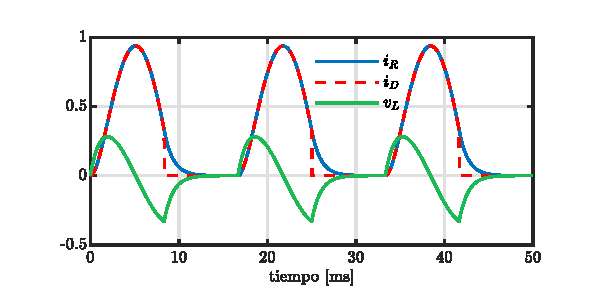
\includegraphics[width=\linewidth]{figuras/ir_id_vl.eps}
    \caption{$i_R$, $i_D$ y $v_L$}
    \label{fig:ir-id-vl}
  \end{subfigure}\hfill
  \begin{subfigure}[t]{0.5\textwidth}
    \centering
    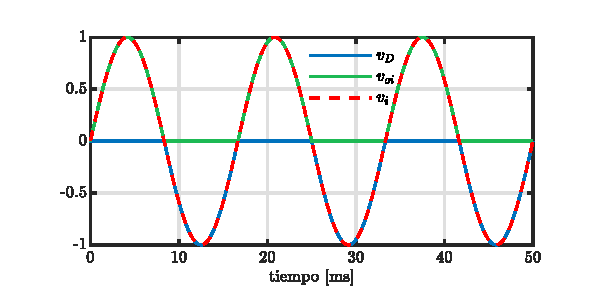
\includegraphics[width=\linewidth]{figuras/voi_vi.eps}
    \caption{$v_{oi}$ y $v_i$}
    \label{fig:voi-vi}
  \end{subfigure}\hfill
  \begin{subfigure}[t]{0.5\textwidth}
    \centering
    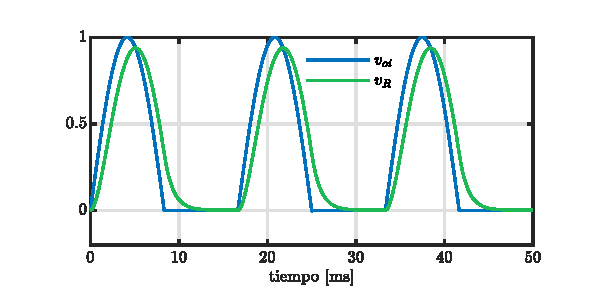
\includegraphics[width=\linewidth]{figuras/voi_vr.eps}
    \caption{$v_{oi}$ y $v_R$}
    \label{fig:voi-vr}
  \end{subfigure}
  \caption{Respuesta del rectificador de media onda con carga $RL$ y diodo de corrida libre.}
  \label{fig:rectificador-subfigs}
\end{figure}






\begin{thebibliography}{plain}
\bibitem{Mohan}
N.~Mohan, T.~M. Undeland y W.~P. Robbins,
\textit{Power Electronics: Converters, Applications, and Design},
3rd ed. Hoboken, NJ, USA: John Wiley \& Sons, 2003.
\bibitem{Rashid}
M.~H. Rashid, \textit{Power Electronics: Circuits, Devices, and Applications},
4th ed. Boston, MA, USA: Pearson, 2014.

\end{thebibliography}

\end{document}